\documentclass{article}

% Encodings, page setup, paragraph formatting, font
\usepackage[top=0.9in, bottom=1in, left=1.5in, right=1.5in]{geometry}
\usepackage[icelandic]{babel}
\usepackage[T1]{fontenc}
\usepackage[sc]{mathpazo}
\usepackage[parfill]{parskip}
\usepackage{cancel}
\usepackage{comment}
% Tables and lists
\usepackage{booktabs,tabularx}
\usepackage{multirow}
\usepackage{enumerate}
\usepackage{adjustbox}
\usepackage{multicol}
\usepackage{enumitem}
\usepackage{xcolor}
% Math
\usepackage{amsmath, amsfonts, amssymb, amsthm}
\usepackage{gensymb}
% Graphics
\usepackage{graphicx}
\usepackage{forest}
\usepackage{tikz}
\usetikzlibrary{positioning, shapes, arrows.meta}
% Code environment
\usepackage{listingsutf8}
\definecolor{commentcolor}{RGB}{0, 128, 0} % Grænn
\definecolor{keywordcolor}{RGB}{0, 0, 255}   % Blár
\definecolor{stringcolor}{RGB}{163, 21, 21}      % Dökkrauður
\definecolor{numbercolor}{RGB}{128, 0, 128}      % Fjólublár
\definecolor{identifiercolor}{RGB}{0, 0, 0}      % Svartur

\def\ojoin{\setbox0=\hbox{$\bowtie$}%
  \rule[-.02ex]{.25em}{.4pt}\llap{\rule[\ht0]{.25em}{.4pt}}}
\def\leftouterjoin{\mathbin{\ojoin\mkern-5.8mu\bowtie}}
\def\rightouterjoin{\mathbin{\bowtie\mkern-5.8mu\ojoin}}
\def\fullouterjoin{\mathbin{\ojoin\mkern-5.8mu\bowtie\mkern-5.8mu\ojoin}}


\lstset{
    language=Java,
    basicstyle=\ttfamily,
    keywordstyle=\color{keywordcolor}\bfseries,
    commentstyle=\color{commentcolor},
    identifierstyle=\color{identifiercolor},
    stringstyle=\color{stringcolor},   
    showstringspaces=false,
    numbers=left,
    numberstyle=\tiny\color{gray},
    tabsize=2,
    breaklines=true,
    columns=fullflexible,
    keepspaces=true,
    inputencoding=utf8, 
    extendedchars=true,  
    literate=
        {á}{{\'a}}1
        {ð}{{\dh}}1
        {é}{{\'e}}1
        {í}{{\'i}}1
        {ó}{{\'o}}1
        {ú}{{\'u}}1
        {ý}{{\'y}}1
        {þ}{{\th}}1
        {æ}{{\ae}}1
        {ö}{{\"o}}1
        {Á}{{\'A}}1
        {Ð}{{\DH}}1
        {É}{{\'E}}1
        {Í}{{\'I}}1
        {Ó}{{\'O}}1
        {Ú}{{\'U}}1
        {Ý}{{\'Y}}1
        {Þ}{{\TH}}1
        {Æ}{{\AE}}1
        {Ö}{{\"O}}1,
}

% Restin af forskriftinni
\usepackage[pdftex,bookmarks=true,colorlinks=true,pdfauthor={Hafsteinn Einarsson},linkcolor=blue,urlcolor=blue]{hyperref}

%Custom Commands til að auðvelda mér lífið
\newcommand{\sv}{\textbf{Svar:}}
\newcommand{\bo}[1]{\textbf{#1}}
\newcommand{\enum}{\begin{enumerate}[label = \alph*.]}

% Hyphenation
\hyphenpenalty=5000
% Page and section numbering
\setcounter{secnumdepth}{-1} 
\pagenumbering{gobble}

\title{Verkefni 2}
\author{brj46 }
\date{vor 2025}

\begin{document}

\maketitle

\vspace{5em}

\begin{center}
    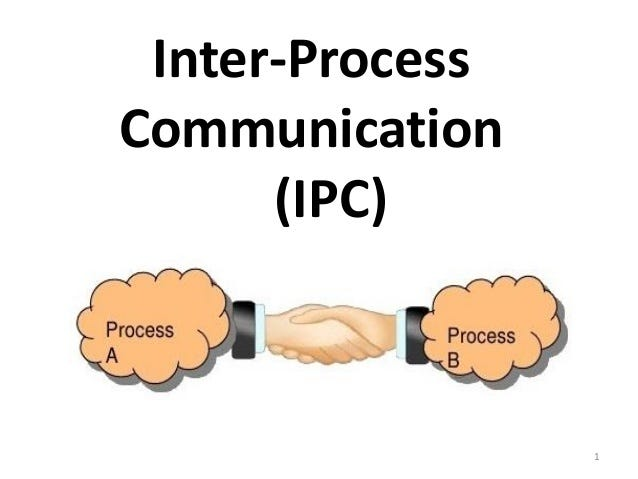
\includegraphics[width=0.6\textwidth]{imgs/IPC.jpeg}
\end{center}

\newpage

\section{1. Introduction to IPC} 
\bo{define interprocess communication and explain why it is essential in operationg systems for enabling processes to work together.}

\sv
interprocess Communication refers to the mechanisms an operating system provides to allow 
processes to share data and coordinate their activities.
Since Processes generally run in seperate adress spaces, interprocess Communication enables
them to cooperate on tasks.
without IPC, processes would be isolated and unable to access shared data or coordinate their activities.


\section{2. Shared Memory}
\bo{ Describe shared memory as a method of IPC where multiple processes can access
the same memory space provided by the operating system.}

\sv
 
Shared memory is an IPC method where the operating system sets aside a region of memory
that multiple processes can access concurrently. Each process that attaches to the shared
memory region can read from and write to this space as if it were a part of its own address space.


\section{3. Message Passing}



\end{document}